\documentclass[a4paper, 12pt]{scrartcl}

\usepackage{scrpage2}
\usepackage[left=2.5cm,right=2.5cm, top=3cm, bottom=4cm]{geometry}
\usepackage[utf8]{inputenc}
\usepackage[ngerman]{babel}
\usepackage[T1]{fontenc}
\usepackage{amsmath}
\usepackage{amssymb}
\usepackage{amsfonts}

\usepackage{graphicx}

%\usepackage{enumerate}
\usepackage[shortlabels]{enumitem}

% Einrücken verhindern
\setlength{\parindent}{0em} 


\begin{document}


\begin{titlepage}
	\centering
	{\Huge\bfseries Versuchsprotokoll\par}
	\vspace{2cm}
	{\scshape\LARGE Mechanik \par}
	\vspace{1cm}
	{\Large Pendel- und Fallexperiment zu Bestimmung der Erdbeschleunigung\par}
	\vfill
	{\large\itshape Simon Schwarz und Marius Ising\par}

	\vfill
\end{titlepage}

\tableofcontents
\newpage

\section{Erdbeschleunigung mit dem Fallexperiment}


\subsection{Versuchsbeschreibung}

Das Ziel des folgenden Versuchs ist die Bestimmung der Erdbeschleunigung $g$. Für eine gleichmäßig beschleunigte Bewegung gilt die Differentialgleichung
$$\ddot s = \frac{d^2s}{dt^2} = a = \mathrm{const}.$$
Durch zweifache Integration erhält man das Weg-Zeit-Gesetz dieser Bewegung
$$s(t) = s_0 + v_0t + \frac a2 t^2.$$
Dabei ist $v_0$ die Anfangsgeschwindigkeit und $s_0$ der anfängliche Weg zum Zeitpunkt $t=0$. Für den betrachteten freien Fall ist dabei die Beschleunigung $a$ gleich der Erdbeschleunigung $g$. Aufgrund der geringen auftretenden Geschwindigkeiten werden zudem Luftreibungseffekte vernachlässigt. Durch eine Weg-Zeit-Messung lässt sich somit $g$ bestimmen.


\subsection{Versuchsaufbau}

\begin{figure}[h]
	\centering
	\includegraphics{Aufbau_ff.jpg}
	\caption{Versuchsaufbau}
\end{figure}
Der Versuchsaufbau dient der Messung der Fallzeit einer Stahlkugel für einstellbare Höhen von 10 bis 90 mm. In eine Grundplatte mit integrierter Auffangplatte wird eine Stativstange mit Skala montiert. Zudem wird eine höhenverstellbare Startkonsole mit Auslösevorrichtung für die Metallkugel an die Stange angebracht. Verlässt die Metallkugel die Haltezunge mit Mikromagnet, so wird ein elektrisches Startsignal ausgelöst. Beim Aufprall auf der Platte entsteht ein Stopp-Signal und die Zeitmessung wird beendet. Die Zeitmessung erfolgt dabei wahlweise mit einem Digital-Zähler oder dem Oszilloskop. Der Zähler und das Oszilloskop werden dabei gleichzeitig angeschlossen.

\begin{figure}[h]
	\centering
	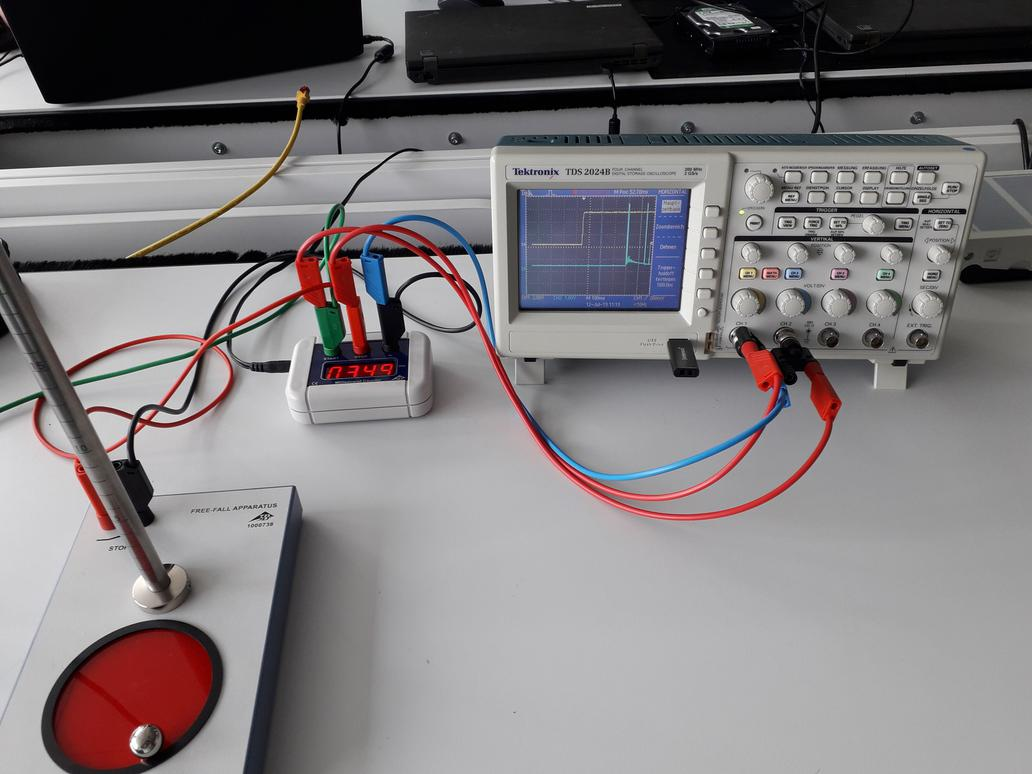
\includegraphics{Aufbau_Detail_ff.jpg}
	\caption{Anschluss von Digital-Zähler und Oszilloskop}
\end{figure}



\subsection{Versuchsdurchführung}

Die Fallzeiten werden für verschiedene Höhen von 10 bis 90 cm in Schritten von 10 cm durchgeführt. Dabei werden für jede Höhe 10 Zeitmessungen mit dem Digitalzähler und eine Messung mit dem Oszilloskop durchgeführt. Das Oszilloskop wird dabei auf Single Seq eingestellt und auf die steigende Flanke des Startsignals getriggert. Das Triggerlevel liegt dabei bei 620 mV. Um eine Startgeschwindidkeit der Kugel zu vermeiden, wird der Auslösebügel möglichst feinfühlig betätigt. Es werden stets alle Messungen für eine Höhe durchgeführt, ehe die Höhe verstellt wird. Bei der Höheneinstellung wird versucht mit der oberen Bohrungskante der Startkonsole genau den Strich der Säulenskala zu treffen.


\subsection{Versuchsauswertung}

Mit dem Digitalzähler ergaben sich folgende Messungen
\begin{table}[h]
\begin{center}
\begin{tabular}{c|r|r|r|r|r|r|r|r|r}
$s$ / cm & 10 & 20 & 30 & 40 & 50 & 60 & 70 & 80 & 90 \\
\hline
$t$ / ms & 140 & 200 & 245 & 284 & 318 & 348 & 376 & 403 & 427 \\
         & 140 & 200 & 246 & 284 & 318 & 348 & 377 & 403 & 427 \\
	 & 140 & 200 & 246 & 284 & 318 & 348 & 376 & 403 & 427 \\
	 & 141 & 200 & 246 & 284 & 318 & 348 & 377 & 403 & 427 \\
	 & 141 & 200 & 246 & 284 & 318 & 348 & 377 & 402 & 407 \\
	 & 141 & 200 & 245 & 284 & 318 & 348 & 376 & 402 & 427 \\
	 & 141 & 200 & 246 & 284 & 318 & 348 & 376 & 402 & 427 \\
	 & 141 & 200 & 245 & 284 & 318 & 348 & 376 & 402 & 427 \\
	 & 141 & 200 & 245 & 284 & 318 & 348 & 376 & 403 & 427 \\
	 & 141 & 200 & 246 & 284 & 318 & 348 & 376 & 402 & 427 \\
\hline
$\bar t$ / ms & 140.7 & 200 & 245.6 & 284 & 318 & 348 & 376.3 & 402.5 & 427
\end{tabular}
\caption{Messreihe mit dem Digitalzähler}
\end{center}
\end{table}

\begin{table}[h]
\begin{center}
\begin{tabular}{c|r|r|r|r|r|r|r|r|r}
$s$ / cm & 10 & 20 & 30 & 40 & 50 & 60 & 70 & 80 & 90 \\
\hline
$t$ / ms & 140.8 & 200 & 245.2 & 283.8 & 318.2 & 348.4 & 376.6 & 402.7 & 427.2 \\
\end{tabular}
\caption{Messreihe mit dem Oszilloskop}
\end{center}
\end{table}

Für die Höhenmessung wird die Unsicherheit auf $\sigma_s = 1 \, \mathrm{mm}$ geschätzt. Aufgrund der geringen statistischen Effekte in der Messreihe der Zeitmessungen mit dem Digitalzähler werden statistische Unsicherheiten vernachlässigt und die Unsicherheit aufgrund der zeitlichen Auflösung des Zählers unter Annahme einer Gleichverteilung zu $\sigma_t = 1/\sqrt{12} \, \mathrm{ms} \approx 0.29 \, \mathrm{ms}$ bestimmt.


\begin{figure}[h]
	\centering
	\includegraphics[scale=0.3]{Auswertung.png}
	\caption{Residuenplots}
\end{figure}




\section{Erdbeschleunigung mit dem Pendel}


\subsection{Versuchsbeschreibung}

In diesem Experiment wird nun die Schwingung eines physikalischen Pendels untersucht, um die Erdbeschleunigung $g$ zu bestimmen. Die Schwingungsgleichung für das physikalische Pendel lautet
$$J \ddot \varphi = - mgl_s \sin(\varphi).$$
Dabei ist $J$ das Gesamtträgheitsmoment des Pendels und $l_s$ der Abstand vom Aufhängepunkt zum Schwerpunkt des Pendels, sowie $\varphi$ der Auslenkwinkel aus der Ruhelage. Auf der rechten Seite der Gleichung steht das rücktreibende Drehmoment, welches durch die Gravitationskraft hervorgerufen wird. Für kleine Winkel, bei denen $\sin(\varphi) \approx \varphi$, ergibt sich eine lineare, homogene Differentialgleichung zweiter Ordnung
$$\ddot \varphi = -\frac{mgl_s}J \varphi.$$
Diese Gleichung hat die allgemeine Lösung
$$\varphi(t) = A\cdot \cos(\omega t)+ B\cdot \sin(\omega t).$$
Die Kreisfrequenz $\omega$ dieser Schwingung ist gegeben durch
$$\omega^2 = \frac{mgl_s}J.$$
Da das Trägheitsmoment $J$ des Pendels schwierig zu bestimmen ist, umgehen wir dieses Problem. Das betrachtete Pendel besteht aus einem Winkelaufnehmer-Profil, der Pendelstange und einem zylindrischen Pendelkörper.

\begin{figure}[h]
	\centering
	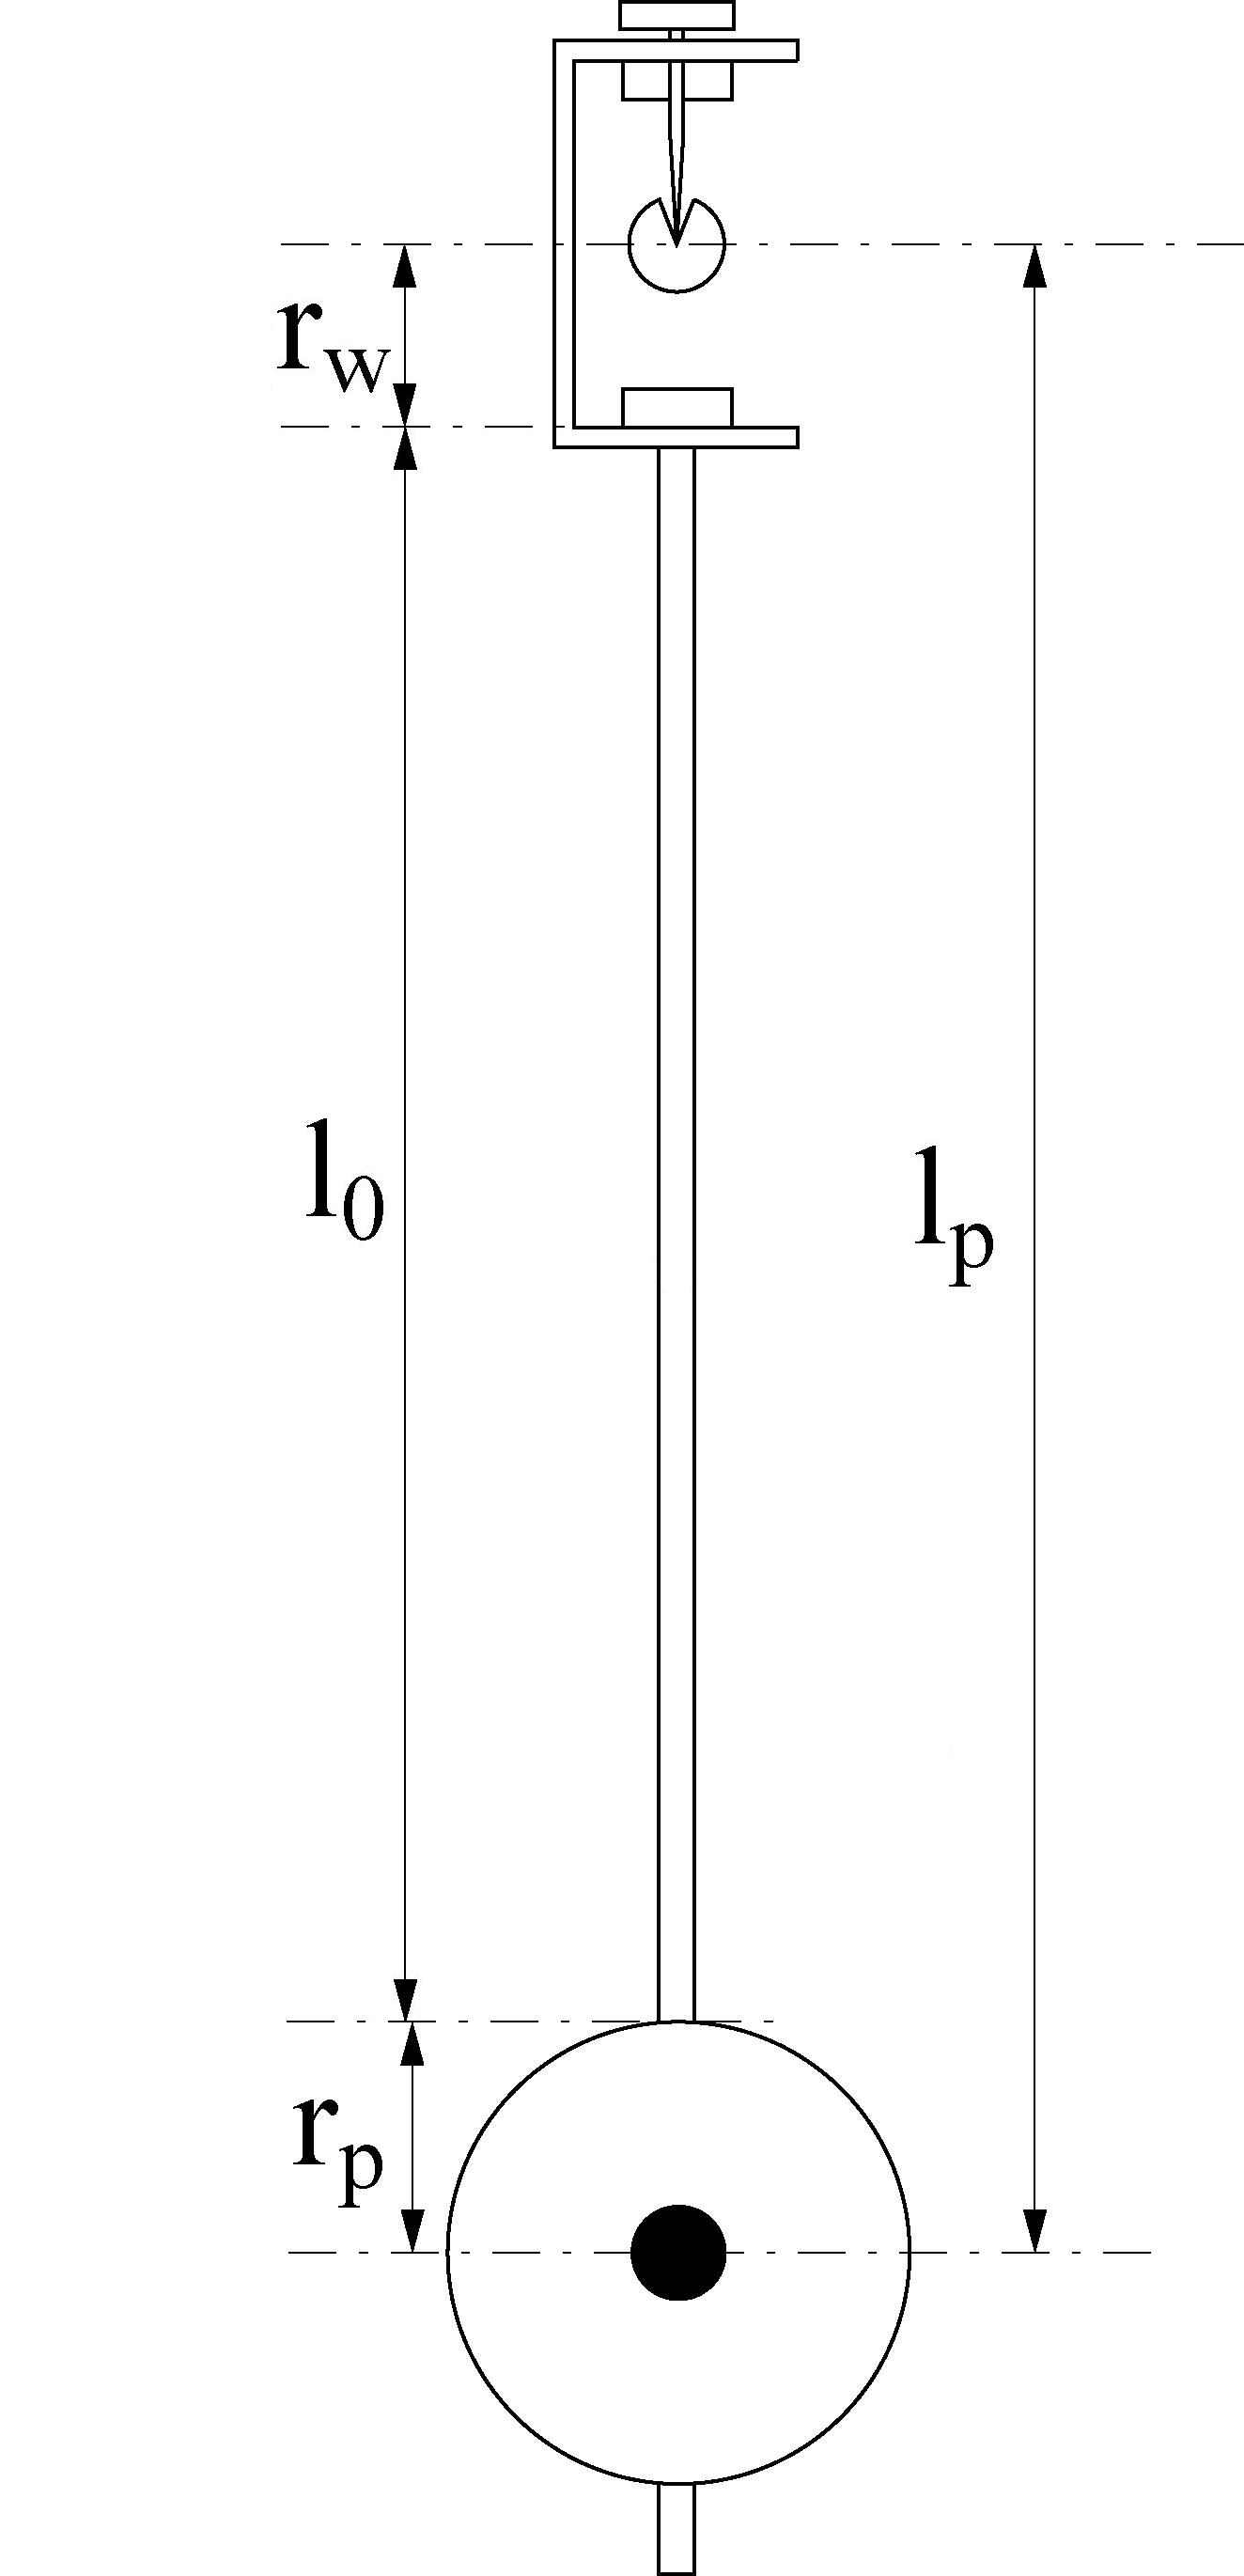
\includegraphics[scale=0.15]{Pendel_Zeichnung_be.jpg}
	\caption{Schematische Zeichung des Pendels}
\end{figure}

Wir bestimmen zunächst die Schwingungsfrequenz $\omega_{st}$ der Stange allein. Anschließend wird der Pendelkörper an der Stelle an der Stange angebracht, an dem das Pendel mit Pendelkörper und Stange diegleiche Schwingungsfrequent hat, wie die Stange allein. Sind $D_{st}$ und $D_p$ die maximalen Rückstellmomente von Stange und Pendelkörper und $J_{st}$ und $J_p$ die entsprechenden Trägheitsmomente, so gilt für die Schwingungfrequenz der Stange allein
$$\omega_{st}^2 = \frac{D_{st}}{J_{st}}.$$
Für den Pendelkörper allein gilt analog
$$\omega_p^2 = \frac{D_p}{J_p}.$$
Da die Rückstellmomente und die Trägheitsmomente additiv sind, ergibt sich die Frequenz des physikalischen Pendels mit Stange und Pendelkörper zu
$$\omega^2 = \frac{D_{st} + D_p}{J_{st} + J_p} = \omega_{st}^2 \frac{1+\frac{D_p}{D_{st}}}{1+\frac{J_p}{J_st}}.$$
Ist der Pendelkörper nun so eingestellt, dass $\omega = \omega_{st}$, so muss $\frac{D_p}{D_{st}} = \frac{J_p}{J_st}$. Daraus erhält man schließlich
$$\omega_p = \omega_{st} = \omega.$$
Das Pendel lässt sich so betrachten als bestünde es nur aus dem Pendelkörper. Mit dem Trägheitsmoment des geometrisch einfachen Pendelkörpers und dem Satz von Steiner ergibt sich
$$J_p = \frac 12 m_p r_p^2 + m_pl_p^2.$$
Damit lässt sich nun die Kreisfrequenz des Pendels ausdrücken
$$\omega^2 = \omega_p^2 = \frac{D_p}{J_p} = \frac{m_pgl_p}{\frac 12 m_pr_p^2+m_pl_p^2}.$$
Durch Umformen folgt schließlich die Formel für die Erdbeschleunigung
$$g = \omega^2l_p \left( 1 + \frac 12 \frac{r_p^2}{l_p^2} \right)$$
Durch Messung des Radius $r_p$ und der Länge $l_p$, sowie der Periodendauer $T = \frac{2\pi}{\omega}$, lässt sich somit die Erdbeschleunigung bestimmen.


\end{document}
